\documentclass{standalone}
\usepackage{tikz}
% start
\usetikzlibrary{intersections}
% end

\begin{document}

% description: intersect vertical and horizontal line
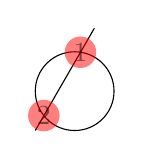
\begin{tikzpicture}
%start
	\draw [name path=a] (0.5,0.5) circle [radius=0.5];
	\draw [name path=b] (0,0) -- (60:1.5);
	\fill [red, opacity=0.5, 
		name intersections={
			of=a and b, 
			name=c
		}]
		(c-1) circle (0.2) node[black] {1}
		(c-2) circle (0.2) node[black] {2};
%end
\end{tikzpicture}

\end{document}
